% \section{Derivation of Strain and SNR Equations}\label{app:strain_snr_deriv}
% In this section we provide a full derivation/explanation of how we arrived at the equations used in our simulations.

% \subsection{Conversions and definitions}
% Each of these conversions and definitions are useful in the later derivations and we define them here for convenience. First, we define the chirp mass of a binary as 
% \begin{equation}\label{eq:chirpmass}
%     \mathcal{M}_c = \frac{(m_1 m_2)^{3/5}}{(m_1 + m_2)^{1/5}},
% \end{equation}
% where $m_1$ and $m_2$ are the primary and secondary mass of the binary. Kepler's third law is well known and allows one to convert between orbital frequency and the semi-major axis of a binary. For convenience we show it here
% \begin{equation}\label{eq:kepler3rd}
%     a = \qty(\frac{G(m_1 + m_2)}{(2 \pi f_{\rm orb})^{2}})^{1/3},\qquad f_{\rm orb} = \frac{1}{2 \pi} \sqrt{\frac{G(m_1 + m_2)}{a^3}}.
% \end{equation}
% As we deal with eccentric binaries, the different harmonic frequencies of gravitational wave emission become important. We therefore write that the relative power radiated into the $n^{\rm th}$ harmonic for a binary with eccentricity $e$ is \citep[][Eq.\,20]{Peters+1963}
% \begin{equation}\label{eq:g(n,e)}
%     \begin{aligned}
%         g(n, e) = \frac{n^{4}}{32} & \left\{ \left[ J_{n-2}(n e)-2 e J_{n-1}(n e)+\frac{2}{n} J_{n}(n e)+2 e J_{n+1}(n e)-J_{n+2}(n e)\right]^{2}\right.\\
%         &\left.+\left(1-e^{2}\right)\left[J_{n-2}(n e)-2 J_{n}(n e)+J_{n+2}(n e)\right]^{2}+\frac{4}{3 n^{2}}\left[J_{n}(n e)\right]^{2}\right\},
%     \end{aligned}
% \end{equation}
% where $J_{n}(v)$ is the Bessel function of the first kind. Thus, the sum of $g(n, e)$ over all harmonics gives the factor by which the gravitational wave emission is stronger for a binary of eccentricity $e$ over an otherwise identical circular binary. This enhancement factor is defined by Peters as \citep[][Eq.\,17]{Peters+1963}
% \begin{equation}\label{eq:eccentricity_enhancement_factor}
%     F(e) = \frac{1 + (73 / 24) e^2 + (37 / 96) e^4}{(1 - e^2)^{7/2}}.
% \end{equation}
% Note that $F(0) = 1$ as one would expect. A fun number to remember is that $F(0.5) \approx 5.0$, or in words, a binary with eccentricity $0.5$ loses energy to gravitational waves at a rate $5$ times higher than a similar circular binary.

% \subsection{Characteristic Strain}
% The characteristic strain from a binary in the $n^{\rm th}$ harmonic is defined as follows (e.g. \citealp[][Eq.\,56]{Barack+2004}; \citealp[][Eq.\,5.1]{ Flanagan+1998})
% \begin{equation}\label{eq:char_strain_dedf}
%     h_{c,n}^2 = \frac{1}{(\pi D_L)^2} \qty( \frac{2 G}{c^3} \frac{\dot{E_n}}{\dot{f_n}} ),
% \end{equation}
% where $D_L$ is the luminosity distance to the binary, $\dot{E}_n$ is the power radiated in the $n^{\rm th}$ harmonic and $\dot{f}_n$ is the rate of change of the $n^{\rm th}$ harmonic frequency. The power radiated in the $n^{\rm th}$ harmonic is given by \citep[][Eq. 19]{Peters+1963}
% \begin{equation}\label{eq:edot_peters}
%     \dot{E}_n = \frac{32}{5} \frac{G^{4}}{c^5} \frac{m_{1}^{2} m_{2}^{2}\left(m_{1}+m_{2}\right)}{a^{5}} g(n, e),
% \end{equation}
% where $m_1$ is the primary mass, $m_2$ is the secondary mass, $a$ is the semi-major axis of the binary and $e$ is the eccentricity. Using \eqref{eq:chirpmass} and \ref{eq:kepler3rd}, we can recast \eqref{eq:edot_peters} in a form more applicable for gravitational wave detections that is a function of only the chirp mass, orbital frequency and eccentricity.
% \begin{align}
%     \dot{E}_n &= \frac{32}{5} \frac{G^{4}}{c^5} \qty(m_{1}^{2} m_{2}^{2}\left(m_{1}+m_{2}\right)) g(n, e) \cdot \qty(\frac{(2 \pi f_{\rm orb})^{2}}{G(m_1 + m_2)})^{5/3} \\
%     \dot{E}_n &= \frac{32}{5} \frac{G^{7/3}}{c^5} \frac{m_{1}^{2} m_{2}^{2}}{\left(m_{1}+m_{2}\right)^{2/3}} (2 \pi f_{\rm orb})^{10/3} g(n, e) \\
%     \dot{E}_n(\mathcal{M}_c, f_{\rm orb}, e) &= \frac{32}{5} \frac{G^{7 / 3}}{c^{5}}\left(2 \pi f_{\mathrm{orb}} \mathcal{M}_{c}\right)^{10 / 3} g(n, e) \label{eq:edot}
% \end{align}
% The last term needed to define the characteristic strain in \eqref{eq:char_strain_dedf} is the rate of change of the $n^{\rm th}$ harmonic frequency. We can first apply the chain rule and note that
% \begin{equation}\label{eq:fdot_chainrule}
%     \dot{f}_{n} = \dv{f_{n}}{a} \dv{a}{t}.
% \end{equation}
% The frequency of the $n^{\rm th}$ harmonic is simply defined as $f_n = n \cdot f_{\rm orb}$ and therefore we can find an expression for $\dd{f_{n}} / \dd{a}$ by rearranging and differentiating \eqref{eq:kepler3rd}
% \begin{align}
%     f_{n} &= \frac{n}{2 \pi} \sqrt{\frac{G(m_1 + m_2)}{a^3}}, \\
%     \dv{f_{n}}{a} &= -\frac{3 n}{4 \pi} \frac{\sqrt{G(m_1 + m_2)}}{a^{5/2}}. \label{eq:dfda}
% \end{align}
% The rate at which the semi-major axis decreases is \citep[][Eq. 5.6]{Peters+1964}
% \begin{equation}\label{eq:dadt}
%     \dv{a}{t} = -\frac{64}{5} \frac{G^{3} m_{1} m_{2}\left(m_{1}+m_{2}\right)}{c^{5} a^{3}} F(e).
% \end{equation}
% Substituting \eqref{eq:dfda} and \ref{eq:dadt} into \eqref{eq:fdot_chainrule} gives an expression for $\dot{f}_{n}$
% \begin{align}
%     \dot{f}_n &= -\frac{3 n}{4 \pi} \frac{\sqrt{G(m_1 + m_2)}}{a^{5/2}} \cdot -\frac{64}{5} \frac{G^{3} m_{1} m_{2}\left(m_{1}+m_{2}\right)}{c^{5} a^{3}} F(e), \\
%     \dot{f}_n &= \frac{48 n}{5 \pi} \frac{G^{7/2}}{c^5} \qty(m_1 m_2 (m_1 + m_2)^{3/2}) \frac{F(e)}{a^{11/2}},
% \end{align}
% which, as above with $\dot{E}_n$, we can recast using Kepler's third law and the definition of the chirp mass
% \begin{align}
%     \dot{f}_n &= \frac{48 n}{5 \pi} \frac{G^{7/2}}{c^5} \qty(m_1 m_2 (m_1 + m_2)^{3/2}) F(e) \cdot \qty(\frac{(2 \pi f_{\rm orb})^{2}}{G(m_1 + m_2)})^{11/6}, \\
%     &= \frac{48 n}{5 \pi} \frac{G^{5/3}}{c^5} \frac{m_1 m_2}{(m_1 + m_2)^{1/3}} \cdot (2 \pi f_{\rm orb})^{11/3} \cdot F(e), \\
%     \dot{f}_n(\mathcal{M}_c, f_{\rm orb}, e) &= \frac{48 n}{5 \pi} \frac{\qty(G \mathcal{M}_c)^{5/3}}{c^5} (2 \pi f_{\rm orb})^{11/3} F(e) \label{eq:fdot}
% \end{align}
% With definitions of both $\dot{E}_n$ and $\dot{f}_n$, we are now in a position to find an expression for the characteristic strain by plugging \eqref{eq:edot} and \ref{eq:fdot} into \ref{eq:char_strain}:
% \begin{align}
%     h^2_{c,n} &= \frac{1}{(\pi D_L)^2} \qty( \frac{2 G}{c^3} \frac{\frac{32}{5} \frac{G^{7 / 3}}{c^{5}}\left(2 \pi f_{\mathrm{orb}} \mathcal{M}_{c}\right)^{10 / 3} g(n, e)}{\frac{48 n}{5 \pi} \frac{\qty(G \mathcal{M}_c)^{5/3}}{c^5} (2 \pi f_{\rm orb})^{11/3} F(e)} ) \\
%     &= \frac{1}{(\pi D_L)^2} \qty( \frac{2^{5/3} \pi^{2/3}}{3} \frac{(G \mathcal{M}_c)^{5/3}}{c^3} \frac{1}{f_{\rm orb}^{1/3}} \frac{g(n, e)}{n F(e)} ) \\
%     h_{c,n}^2(\mathcal{M}_c, D_L, f_{\rm orb}, e) &= \frac{2^{5/3}}{3 \pi^{4/3}} \frac{(G \mathcal{M}_c)^{5/3}}{c^3 D_L^2} \frac{1}{f_{\rm orb}^{1/3}} \frac{g(n, e)}{n F(e)} \label{eq:char_strain}
% \end{align}

% \subsection{Strain}
% The strain can be found by dividing the characteristic strain by the square root of twice the number of cycles. This is explained in \citet{Finn+2000} and in further detail in \citet{Moore+2015}. The physical reasoning behind the idea is that the binary will spend a certain amount of time in the vicinity of some frequency $f$ and cause a similar gravitational wave strain. This leads to the signal 'accumulating' and resulting in a larger signal-to-noise ratio. Therefore, the characteristic strain represents the strain measured by the detector over the duration of the mission, whilst the strain is what is emitted by the binary at each instantaneous moment.

% Following this logic, we can convert between characteristic strain and strain with \citep[e.g][see text before Eq.\,2.2]{Finn+2000}
% \begin{equation}\label{eq:strain-to-charstrain}
%     h_{c, n}^2 = \qty(\frac{2 f_n^2}{\dot{f}_n}) h_n^2.
% \end{equation}
% Therefore, using this, in addition to Eq. \ref{eq:fdot} and Eq. \ref{eq:char_strain}, we can write an expression for the strain amplitude of gravitational waves in the $n^{\rm th}$ harmonic
% \begin{align}
%     h_n^2 &= \qty(\frac{\dot{f}_n}{2 f_n^2}) h_{c, n}^2, \\
%     h_n^2 &= \qty(\frac{48 n}{5 \pi} \frac{\qty(G \mathcal{M}_c)^{5/3}}{c^5} (2 \pi f_{\rm orb})^{11/3} F(e) \cdot \frac{1}{2 n^2 f_{\rm orb}^2}) \qty(\frac{2^{5/3}}{3 \pi^{4/3}} \frac{(G \mathcal{M}_c)^{5/3}}{c^3 D_L^2} \frac{1}{n f_{\rm orb}^{1/3}} \frac{g(n, e)}{F(e)}), \\
%     h_n^2(\mathcal{M}_c, f_{\rm orb}, D_L, e) &= \frac{2^{25/3}}{5} \frac{(G \mathcal{M}_c)^{10/3}}{c^8 D_L^2} \frac{g(n, e)}{n^2} \qty(\pi f_{\rm orb})^{4/3} . \label{eq:strain}
% \end{align}

% \subsection{General Signal-to-Noise Ratio}
% We can start at the equation for the general signal-to-noise ratio from \citet{Flanagan+1998} (Eq. 2.30)
% \begin{equation}
%     \left\langle\rho^{2}\right\rangle=\frac{2(1+z)^{2}}{5 \pi^{2} D_L(z)^{2}} \int_{0}^{\infty} d f \frac{1}{f^{2} S_{n}(f)} \dv{E}{f}[(1 + z) f],
% \end{equation}
% where $z$ is the redshift. We need to adjust this equation in a couple of key ways for LISA Galactic binaries. First we multiply by 5 because of the way the signal response function is defined in LISA (converse to LIGO) -- \citet[see][]{Robson+2019} for a good explanation. Additionally we can set $z = 0$ for Galactic binaries, convert to SI units from geometric units (as is our convention in this document) and integrate over specific frequency limits.
% \begin{equation}\label{eq:snr_abs}
%     \avg{\rho_n^2} = \int_{f_{n, i}}^{f_{n, f}} \underbrace{\frac{2 G}{\pi^2 c^3 D_L^2} \dv{E_n}{f_n}}_{\text{signal}} \underbrace{\frac{1}{f_n^2 S_{\rm n}(f_n)}}_{\text{noise}} \dd{f_n}.
% \end{equation}
% It is now useful to inspect the `signal' term in the equation. We can do this specifically by first finding an expression for $\dd{E_n}/\dd{f_n}$ through the chain rule. We can write
% \begin{equation}\label{eq:dedf}
%     \dv{E_n}{f_n} = \dv{E_n}{t} \dv{a}{f_n} \dv{t}{a},
% \end{equation}
% where each term respectively comes from \eqref{eq:edot_peters}, the inverse of \eqref{eq:dfda} and the inverse of \eqref{eq:dadt}.
% We can substitute these into Eq. \ref{eq:dedf} and simplify as follows
% \begin{align}
%     \dv{E_n}{f_n} &= \frac{32}{5} \frac{G^{4}}{c^5} \frac{m_1^2 m_2^2 \qty(m_1 + m_2)}{a^5} g(n, e) \cdot -\frac{4 \pi}{3 n} \frac{a^{5/2}}{(G(m_1 + m_2))^{1/2}} \cdot -\frac{5}{64} \frac{c^5 a^3}{G^3 m_1 m_2 (m_1 + m_2)} \frac{1}{F(e)}, \\
%     &= \frac{2 \pi}{3} \frac{G^{1/2} m_1 m_2}{(m_1 + m_2)^{1/2}} \frac{g(n, e)}{n F(e)} \cdot a^{1/2}, \\
%     &= \frac{2 \pi}{3} \frac{G^{1/2} m_1 m_2}{(m_1 + m_2)^{1/2}} \frac{g(n, e)}{n F(e)} \cdot \qty(\frac{G(m_1 + m_2)}{(2 \pi f_{\rm orb})^2})^{1/6}, \\
%     &= \frac{2^{2/3} \pi^{2/3}}{3} \frac{G^{2/3} m_1 m_2}{(m_1 + m_2)^{1/3}} \frac{g(n, e)}{n F(e)} \cdot f_{\rm orb}^{-1/3}, \\
%     \dv{E_n}{f_n} &= \frac{2^{2/3} \pi^{2/3}}{3} G^{2/3} \mathcal{M}^{5/3} \frac{g(n, e)}{n F(e)} \cdot f_{\rm orb}^{-1/3}.
% \end{align}
% If we further multiply this by the prefactor in \eqref{eq:snr_abs}, we arrive at an expression for the `signal' portion of the equation, which notably is exactly the square of the characteristic strain (see \eqref{eq:char_strain}).
% \begin{equation}
%     \dv{E_n}{f_n} \frac{2 G}{\pi^2 c^3 D_L^2} = \frac{2^{5/3} }{3 \pi^{4/3}} \frac{(G \mathcal{M}_c)^{5/3}}{c^3 D_L^2} \frac{1}{n f_{\rm orb}^{1/3}} \frac{g(n, e)}{F(e)} = h_{c,n}^2.
% \end{equation}
% We can therefore write that the sky-averaged signal-to-noise ratio for a Galactic binary is
% \begin{equation}\label{eq:snr_general}
%     \boxed{ \rho^2 = \sum_{n=1}^{\infty}  \int_{f_{n, i}}^{f_{n, f}} \frac{h_{c, n}^2}{f_n^2 S_{\rm n}(f_n)} \dd{f_n}. }
% \end{equation}

% \subsection{Stationary Signal-to-Noise Ratio}
% For our sample, it was extremely useful to note that the vast majority of our binaries were stationary in frequency space on the timescale of a space-based observing mission. In this case, the start and end frequencies are only separated by a very small $\Delta f_n$ and so we can make the approximation that
% \begin{align}
%     \rho_n^2 &= \lim_{\Delta f \to 0} \int_{f_{n}}^{f_{n} + \Delta f_n} \frac{h_{c, n}^2}{f_n^2 S_n(f_n)} \dd{f_n}, \nonumber \\
%     &\approx \frac{\Delta f_n \cdot h_{c, n}^2}{f_n^2 S_n(f_n)}.
% \end{align}
% Moreover, we can immediately write that $\Delta f_n = \dot{f}_n \Delta T$, where we know that $\Delta T = T_{\rm obs}$, such that
% \begin{equation}
%     \rho_n^2 = \left(\frac{\dot{f}_n}{f_n^2} h_{c, n}^2 \right) \frac{T_{\rm obs}}{S_n(f_n)},
% \end{equation}
% where the term in parentheses can be replaced with $2 h_n^2$ using Equation \ref{eq:strain-to-charstrain}. This gives the final expression for the signal-to-noise ratio when the stationary approximation is applied (as shown in Equation \ref{eq:snr_stat})
% \begin{equation}
%     \rho_{\rm stat}^2 = \sum_{n=1}^{\infty} \frac{2 T_{\rm obs} h_n^2}{S_n(f_n)} .
% \end{equation}

\section{Detection Rate Normalisation}\label{app:rate_normalisation}
From each instance of the Milky Way that we simulate we can extract the number of targets\footnote{By targets, we are referring to either BHBH, BHNS or NSNS that merge in a Hubble time} that are detectable. However, this number must be normalised in order to show the true detection rate for the Milky Way. Therefore, we write that the number of detectable targets in the Milky Way is
\begin{equation}\label{eq:norm_frame}
    N_{\rm detect} = f_{\rm detect} \cdot N_{\rm target, MW},
\end{equation}
where $f_{\rm detect}$ is the fraction of targets in the instance that were detectable and $N_{\rm target, MW}$ is the total number of targets that have been formed in the Milky Way's history. We can find this total in two steps: (1) find the average number of targets formed per star forming mass (2) find the total star forming mass that has existed in the Milky Way's history.

\subsection{Average target formation rate}
Since double compact object formation is strongly metallicity dependent, we can find the average rate as the integral over metallicity
\begin{equation}\label{eq:norm_avg_target_formation}
    \avg{ \mathcal{R}_{\rm target} } = \int_{Z_{\rm min}}^{Z_{\rm max}} p_{Z} \mathcal{R}_{\rm target, Z} \dd{Z},
\end{equation}
where $Z_{\rm min}, Z_{\rm max}$ are the minimum and maximum sampled metallicities, $p_Z$ is the probability of forming a star at the metallicity $Z$ \citep{Frankel+2018} and $\mathcal{R}_{\rm target, Z}$ is defined as the number of targets formed per star forming mass. 
\begin{equation}
    \mathcal{R}_{\rm target, Z} =  N_{\rm target, Z} / M_{\rm SF, Z}.
\end{equation}
The number of targets in our sample at a metallicity $Z$ can be written simply as the sum of the targets' weights:
\begin{equation}
    N_{\rm target, Z} = \sum_{i=1}^{N_{\rm binaries, Z}} w_i \theta_{\rm target, i},
\end{equation}
where $w_i$ is the STROOPWAFEL weight assigned to a binary, $N_{\rm binaries, Z}$ is the number of binaries at metallicity $Z$ in our sample and $\theta_{\rm target, i}$ is a step function that is only $1$ when the binary is a target and otherwise 0. The total star forming mass at a metallicity $Z$ can be written as
\begin{equation}
    M_{\rm SF, Z} = \frac{\avg{m}_{\rm COMPAS, Z}}{f_{\rm trunc}} \sum_{i=1}^{N_{\rm binaries, Z}} w_i,
\end{equation}
where $\avg{m}_{\rm COMPAS}$ is the average star forming mass of a binary in our sample and $f_{\rm trunc}$ is the fraction of the total stellar mass that COMPAS samples from given its truncated mass and separation ranges (see Section \ref{sec:COMPAS_explained}). The cuts applied to the distributions mean that only $f_{\rm trunc} \approx 0.2$ of the stellar mass is sampled from.

\subsection{Total star forming mass in the Milky Way}
It is important to distinguish between the \textit{total} star forming mass in the Milky Way and the \textit{current} star forming mass in the Milky Way. Many stars born in the Milky Way are no longer living and have lost much of their mass to stellar winds and supernovae, thus decreasing the total stellar mass. \citet{Licquia+2015} find that the total stellar mass today in the Milky Way disc is $6.08 \pm 1.14 \times 10^{10} \unit{M_{\rm odot}}$. This total includes all stars and stellar remnants (white dwarfs, neutrons stars and black holes) but \textit{excludes} brown dwarfs. We can write that the total star forming mass that has \textit{ever} existed in the Milky Way is
\begin{equation}\label{eq:m_SF_MW}
    M_{\rm SF, MW} = 6.08 \pm 1.14 \times 10^{10} \unit{M_{\rm odot}} \cdot \frac{\avg{m}_{\rm SF, total}}{\avg{m}_{\rm SF, today}},
\end{equation}
where $\avg{m}_{\rm SF, total}$ is the average star forming mass over the history of the Milky Way and $\avg{m}_{\rm SF, today}$ is the average star forming mass of the mass remaining today. The former is defined as
\begin{equation}
    \avg{m}_{\rm SF, total} = \int_{0}^{t_{\rm MW}} p_{\rm birth}(t) \int_{0.01}^{200} \zeta(m)\ m \dd{m} \dd{t},
\end{equation}
where $t_{\rm MW}$ is the age of the Milky Way, $\zeta(m)$ is the \citet{Kroupa+2001} IMF function and $p_{\rm birth}(\tau)$ is the probability of a star being formed at a lookback time $\tau$ \citep[][Eq.\,4]{Frankel+2018}. The average star forming mass of the mass \textit{remaining today} is defined as follows (note that we integrate from $0.08$ not $0.01$ since observations of today's Milky Way mass exclude brown dwarfs)
\begin{equation}
    \avg{m}_{\rm SF, today} = \int_{0}^{t_{\rm MW}} p_{\rm birth}(\tau) \int_{0.08}^{200} \zeta(m)\ m_{\rm today}(m, \avg{Z}_\tau, \tau) \dd{m} \dd{\tau},
\end{equation}
where $m_{\rm today}(m, Z, \tau)$ is the mass of a star that was formed $\tau$ years ago at a metallicity $Z$. We calculate this by interpolating a grid of single stars in COMPAS over different masses and metallicities and seeing what final mass they get using the \citet{Fryer+2012} delayed prescription and default wind mass loss settings. We only use the final mass if more than $\tau_{\rm MS}(m, Z)$ main sequence lifetime of the star has passed, otherwise we just use the initial mass. Since we don't know the exact metallicity of each star we use the average metallicity in the Milky Way at a lookback time $\tau$ using the birth radius distribution and metallicity equation from \citet{Frankel+2018}. If we now evaluate Equation \ref{eq:m_SF_MW}, we find the that total star forming mass that ever existed in the Milky Way is
\begin{equation}
    M_{\rm SF, MW} = 6.1 \pm 1.1 \times 10^{10} \unit{M_{\odot}} \cdot \frac{0.384 \unit{M_{\odot}}}{0.257 \unit{M_{\odot}}} = 9.1 \pm 1.1 \times 10^{10} \unit{M_{\odot}},
\end{equation}
an increase of approximately 50\% from the value still in stars today.

\subsection{Normalisation summary}
We can plug Equations~\ref{eq:norm_avg_target_formation} and \ref{eq:m_SF_MW} into \ref{eq:norm_frame} and write that the overall normalisation of the detection rate is calculated as
\begin{equation}
    N_{\rm detect} = 9.1 \times 10^{10} \unit{M_{\odot}} \cdot f_{\rm detect} \cdot \sum_{Z=Z_{\rm min}}^{Z_{\rm max}} p_{Z} \qty(\sum_{i=1}^{N_{\rm binaries, Z}} w_i \theta_{\rm target, i}) \qty(\frac{\avg{m}_{\rm COMPAS, Z}}{f_{\rm trunc}} \sum_{i=1}^{N_{\rm binaries, Z}} w_i)^{-1}
\end{equation}

\section{Supplementary material}

\subsection{Detection rate table}
\begin{table*}[htb]
    \centering
    \caption{The number of detectable binaries in a 4 and 10 year LISA mission for the 15 different model variations and each DCO type. Each value shows the median and the 90\% confidence interval.}
    \begin{tabular}{c|lll|lll}
        \hline
        \multirow{2}{*}{Model} & \multicolumn{3}{c|}{LISA (4 year)} & \multicolumn{3}{c}{LISA (10 year)} \\ \cline{2-7}
         & \scriptsize{BHBH} & \scriptsize{BHNS} & \scriptsize{NSNS} & \scriptsize{BHBH} & \scriptsize{BHNS} & \scriptsize{NSNS} \\
        \hline
        A & \confinv{34.4}{20.9}{46.6} & \confinv{29.9}{20.1}{47.4} & \confinv{7.7}{5.0}{10.3} & \confinv{58.6}{31.0}{53.3} & \confinv{51.9}{28.0}{95.0} & \confinv{13.0}{6.8}{14.2}\\
        B & \confinv{33.9}{19.7}{36.5} & \confinv{15.5}{9.6}{19.6} & \confinv{2.8}{1.9}{4.3} & \confinv{55.6}{27.7}{45.9} & \confinv{26.7}{13.8}{23.7} & \confinv{4.8}{2.7}{5.6}\\
        C & \confinv{20.6}{11.1}{20.5} & \confinv{5.3}{3.0}{5.3} & \confinv{4.3}{3.1}{5.2} & \confinv{33.7}{15.7}{26.7} & \confinv{8.9}{4.2}{7.0} & \confinv{7.3}{4.5}{6.1}\\
        D & \confinv{21.9}{14.7}{37.8} & \confinv{4.1}{2.6}{4.2} & \confinv{11.6}{8.3}{22.7} & \confinv{36.0}{21.6}{45.4} & \confinv{6.8}{3.4}{5.3} & \confinv{20.5}{12.7}{27.7}\\
        E & \confinv{33.7}{19.4}{37.0} & \confinv{3.3}{2.3}{6.3} & \confinv{0.2}{0.1}{0.1} & \confinv{54.9}{26.7}{44.2} & \confinv{5.8}{3.5}{8.2} & \confinv{0.3}{0.1}{0.2}\\
        F & \confinv{26.2}{16.0}{35.8} & \confinv{15.0}{11.4}{84.0} & \confinv{5.7}{3.8}{7.3} & \confinv{43.3}{22.2}{43.7} & \confinv{27.2}{18.2}{86.3} & \confinv{9.5}{5.2}{10.0}\\
        G & \confinv{29.5}{15.9}{27.6} & \confinv{23.5}{14.0}{27.2} & \confinv{23.4}{15.2}{27.9} & \confinv{47.5}{21.4}{38.3} & \confinv{40.9}{20.7}{36.3} & \confinv{39.8}{21.4}{36.3}\\
        H & \confinv{115.1}{98.0}{123.0} & \confinv{30.7}{21.4}{163.7} & \confinv{7.4}{4.8}{14.6} & \confinv{173.6}{117.7}{150.5} & \confinv{55.4}{32.8}{185.8} & \confinv{13.0}{6.8}{25.5}\\
        I & \confinv{22.7}{12.4}{26.8} & \confinv{48.7}{30.9}{97.1} & \confinv{6.3}{4.0}{9.0} & \confinv{36.1}{16.8}{30.8} & \confinv{84.0}{45.0}{142.8} & \confinv{10.9}{5.8}{11.1}\\
        J & \confinv{47.5}{31.6}{71.9} & \confinv{24.3}{16.3}{37.4} & \confinv{6.8}{4.4}{10.9} & \confinv{80.7}{46.8}{86.8} & \confinv{41.7}{22.9}{47.0} & \confinv{11.6}{6.2}{14.0}\\
        K & \confinv{30.1}{18.0}{40.4} & \confinv{37.6}{24.6}{44.9} & \confinv{7.8}{5.1}{11.6} & \confinv{52.5}{28.2}{48.4} & \confinv{65.1}{35.0}{54.7} & \confinv{13.4}{7.1}{14.8}\\
        L & \confinv{35.2}{21.3}{45.2} & \confinv{30.2}{19.9}{49.6} & \confinv{7.9}{5.0}{11.7} & \confinv{58.9}{31.0}{54.9} & \confinv{52.4}{28.5}{96.9} & \confinv{13.3}{7.1}{14.8}\\
        M & \confinv{43.0}{28.3}{58.3} & \confinv{68.7}{43.4}{108.7} & \confinv{16.1}{10.4}{20.5} & \confinv{69.4}{38.1}{69.1} & \confinv{117.4}{61.8}{154.5} & \confinv{27.3}{14.5}{26.4}\\
        N & \confinv{53.0}{34.1}{58.3} & \confinv{110.6}{71.3}{193.1} & \confinv{35.7}{23.6}{54.8} & \confinv{84.4}{44.9}{73.3} & \confinv{194.9}{102.6}{256.0} & \confinv{60.2}{32.7}{67.8}\\
        O & \confinv{43.1}{27.0}{39.0} & \confinv{76.0}{43.9}{91.2} & \confinv{9.3}{6.0}{10.4} & \confinv{68.5}{35.8}{47.5} & \confinv{130.8}{62.9}{122.0} & \confinv{15.8}{8.4}{13.8}\\
        P & \confinv{44.3}{28.4}{62.2} & \confinv{26.7}{17.0}{48.9} & \confinv{9.0}{5.6}{10.9} & \confinv{69.9}{38.0}{78.9} & \confinv{45.9}{25.9}{64.4} & \confinv{15.3}{7.4}{13.9}\\
        Q & \confinv{0.0}{0.0}{0.0} & \confinv{6.3}{3.7}{6.1} & \confinv{7.8}{4.7}{8.0} & \confinv{0.0}{0.0}{0.0} & \confinv{10.8}{5.3}{7.6} & \confinv{13.0}{6.4}{10.4}\\
        \hline
    \end{tabular}
    \label{tab:detection_rates}
\end{table*}

\subsection{Physics variation cumulative distributions}

\begin{figure*}[h]
    \centering
    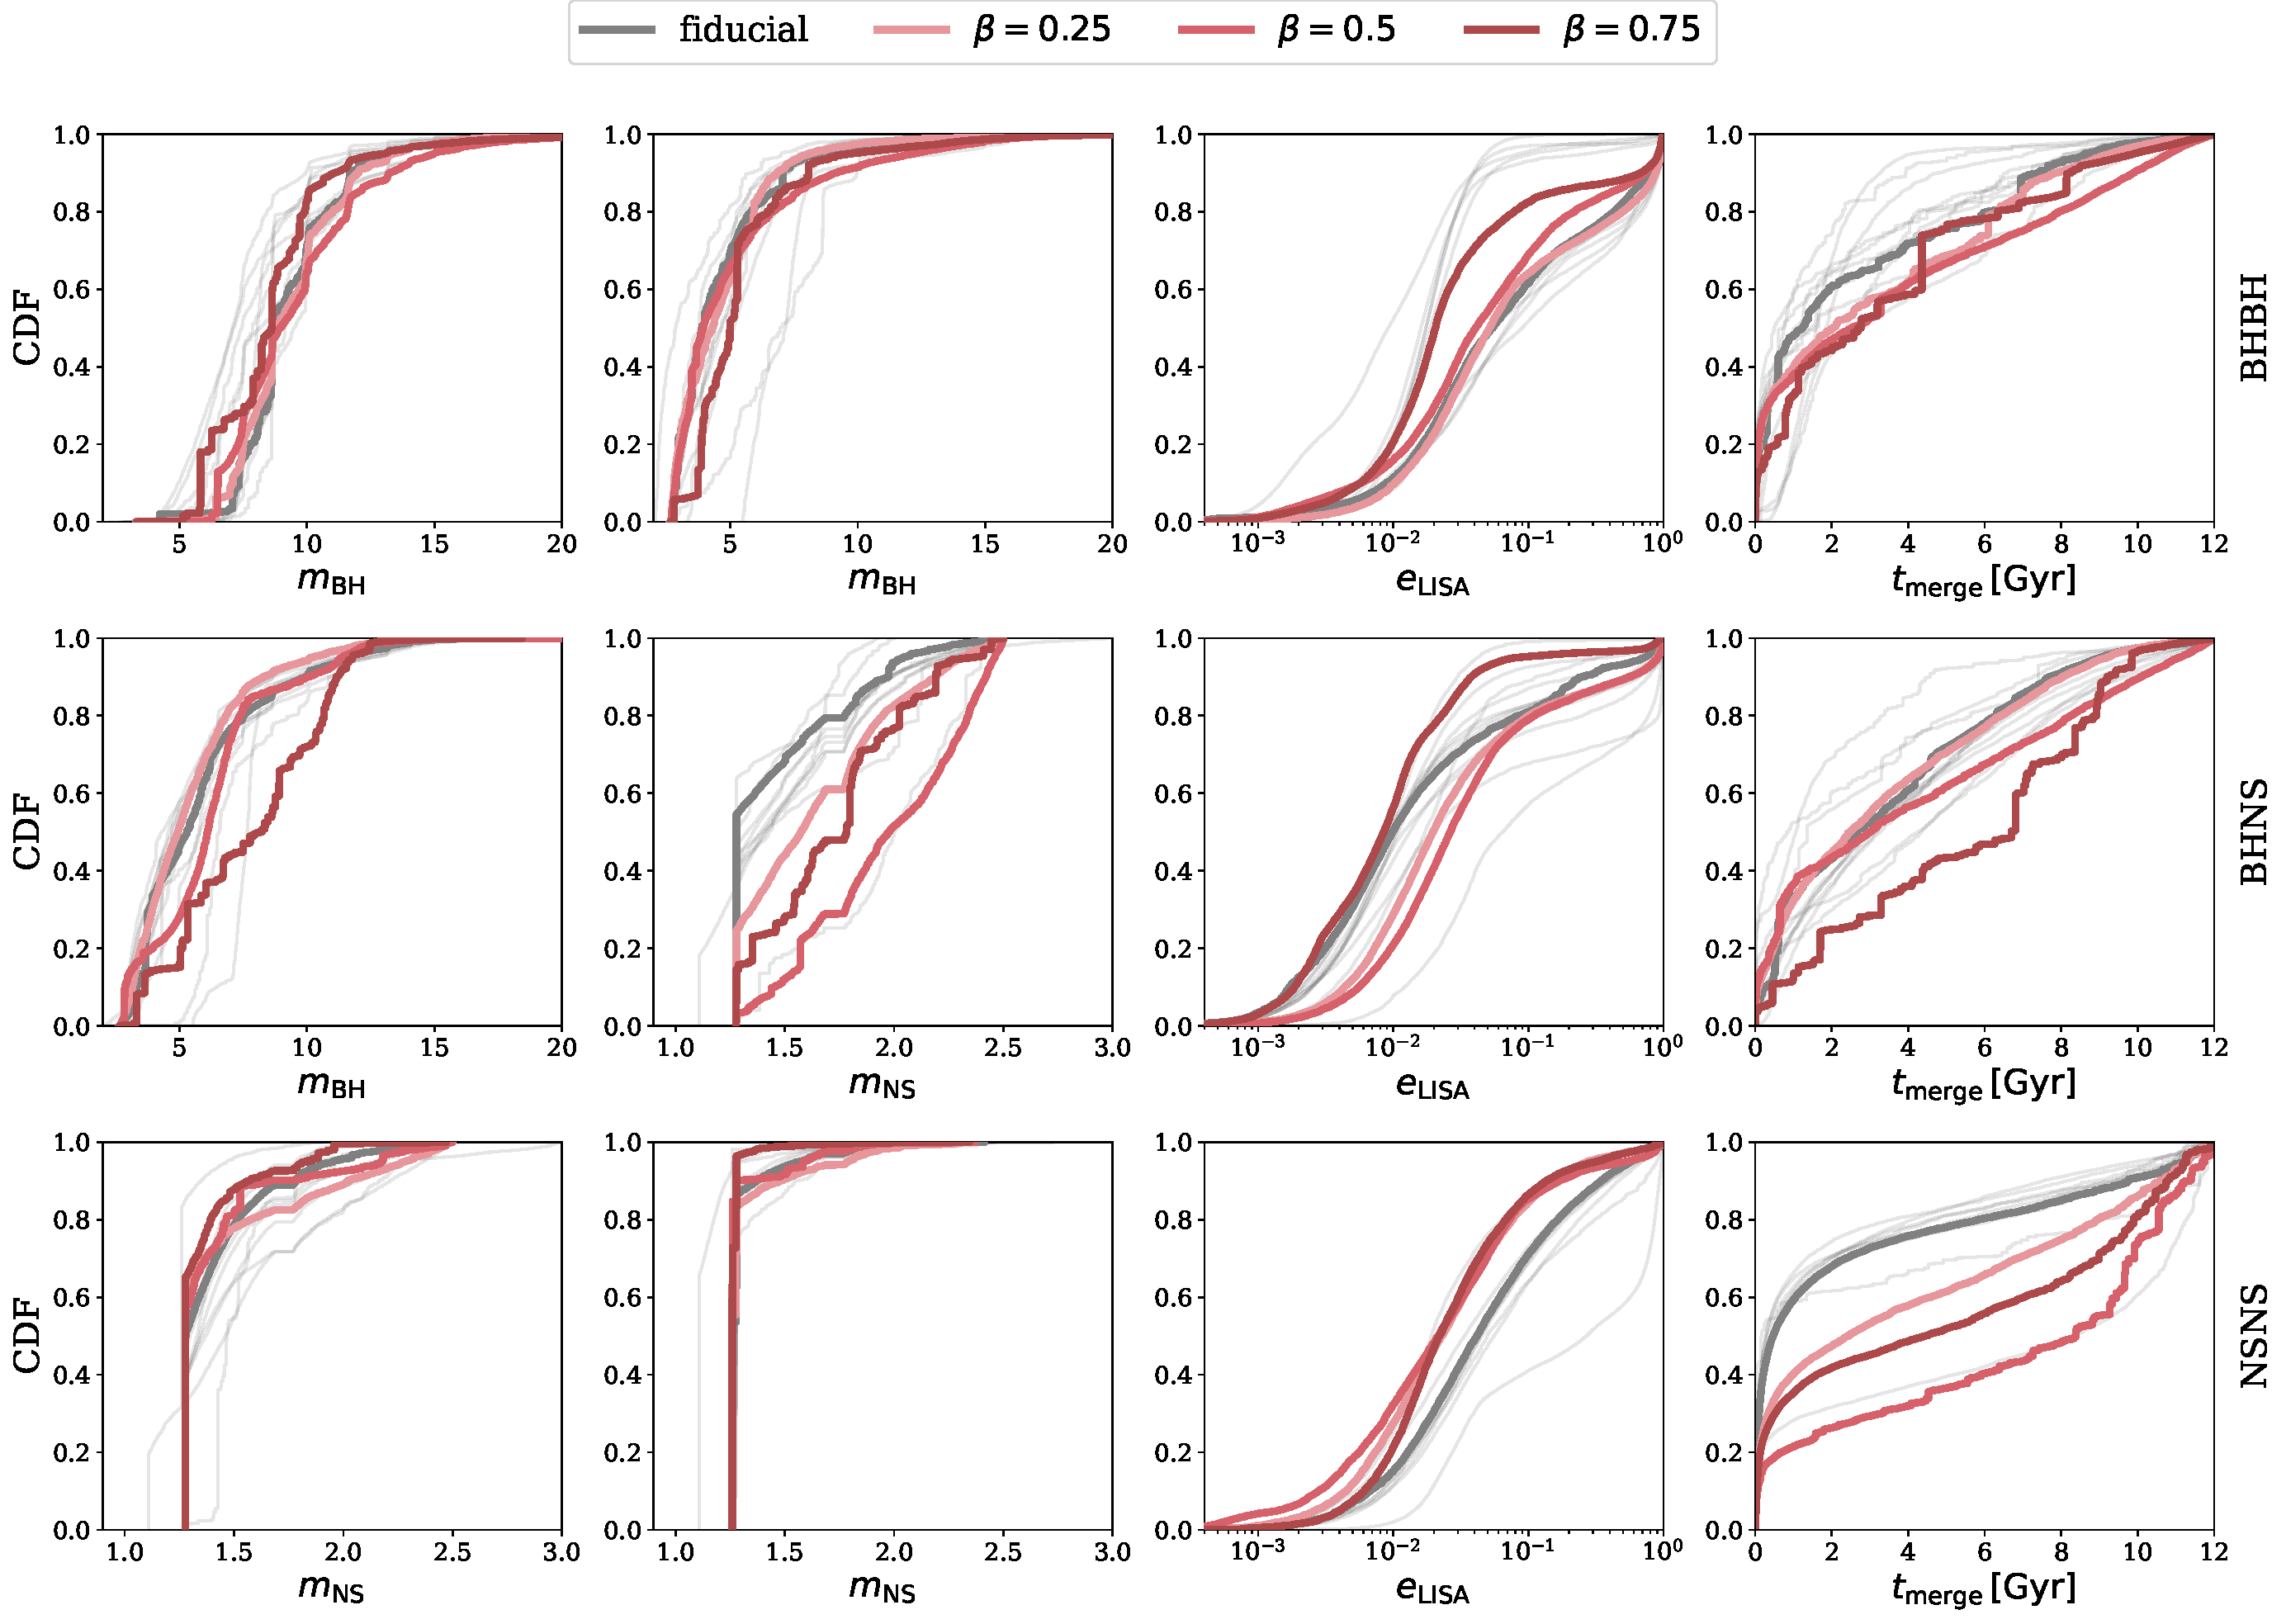
\includegraphics[width=\textwidth]{variations_cdf_1_3.pdf}
    \caption{Cumulative distribution functions for the black hole mass, neutron star mass, eccentricity during the LISA mission and merger time for each DCO type and physics variation. In colour we show the fiducial populations compared to changing the mass transfer efficiency $\beta$. We additionally show the other physics variations in the background in light grey.}
    \label{fig:variations_cdf_1_3}
\end{figure*}

\begin{figure*}[h]
    \centering
    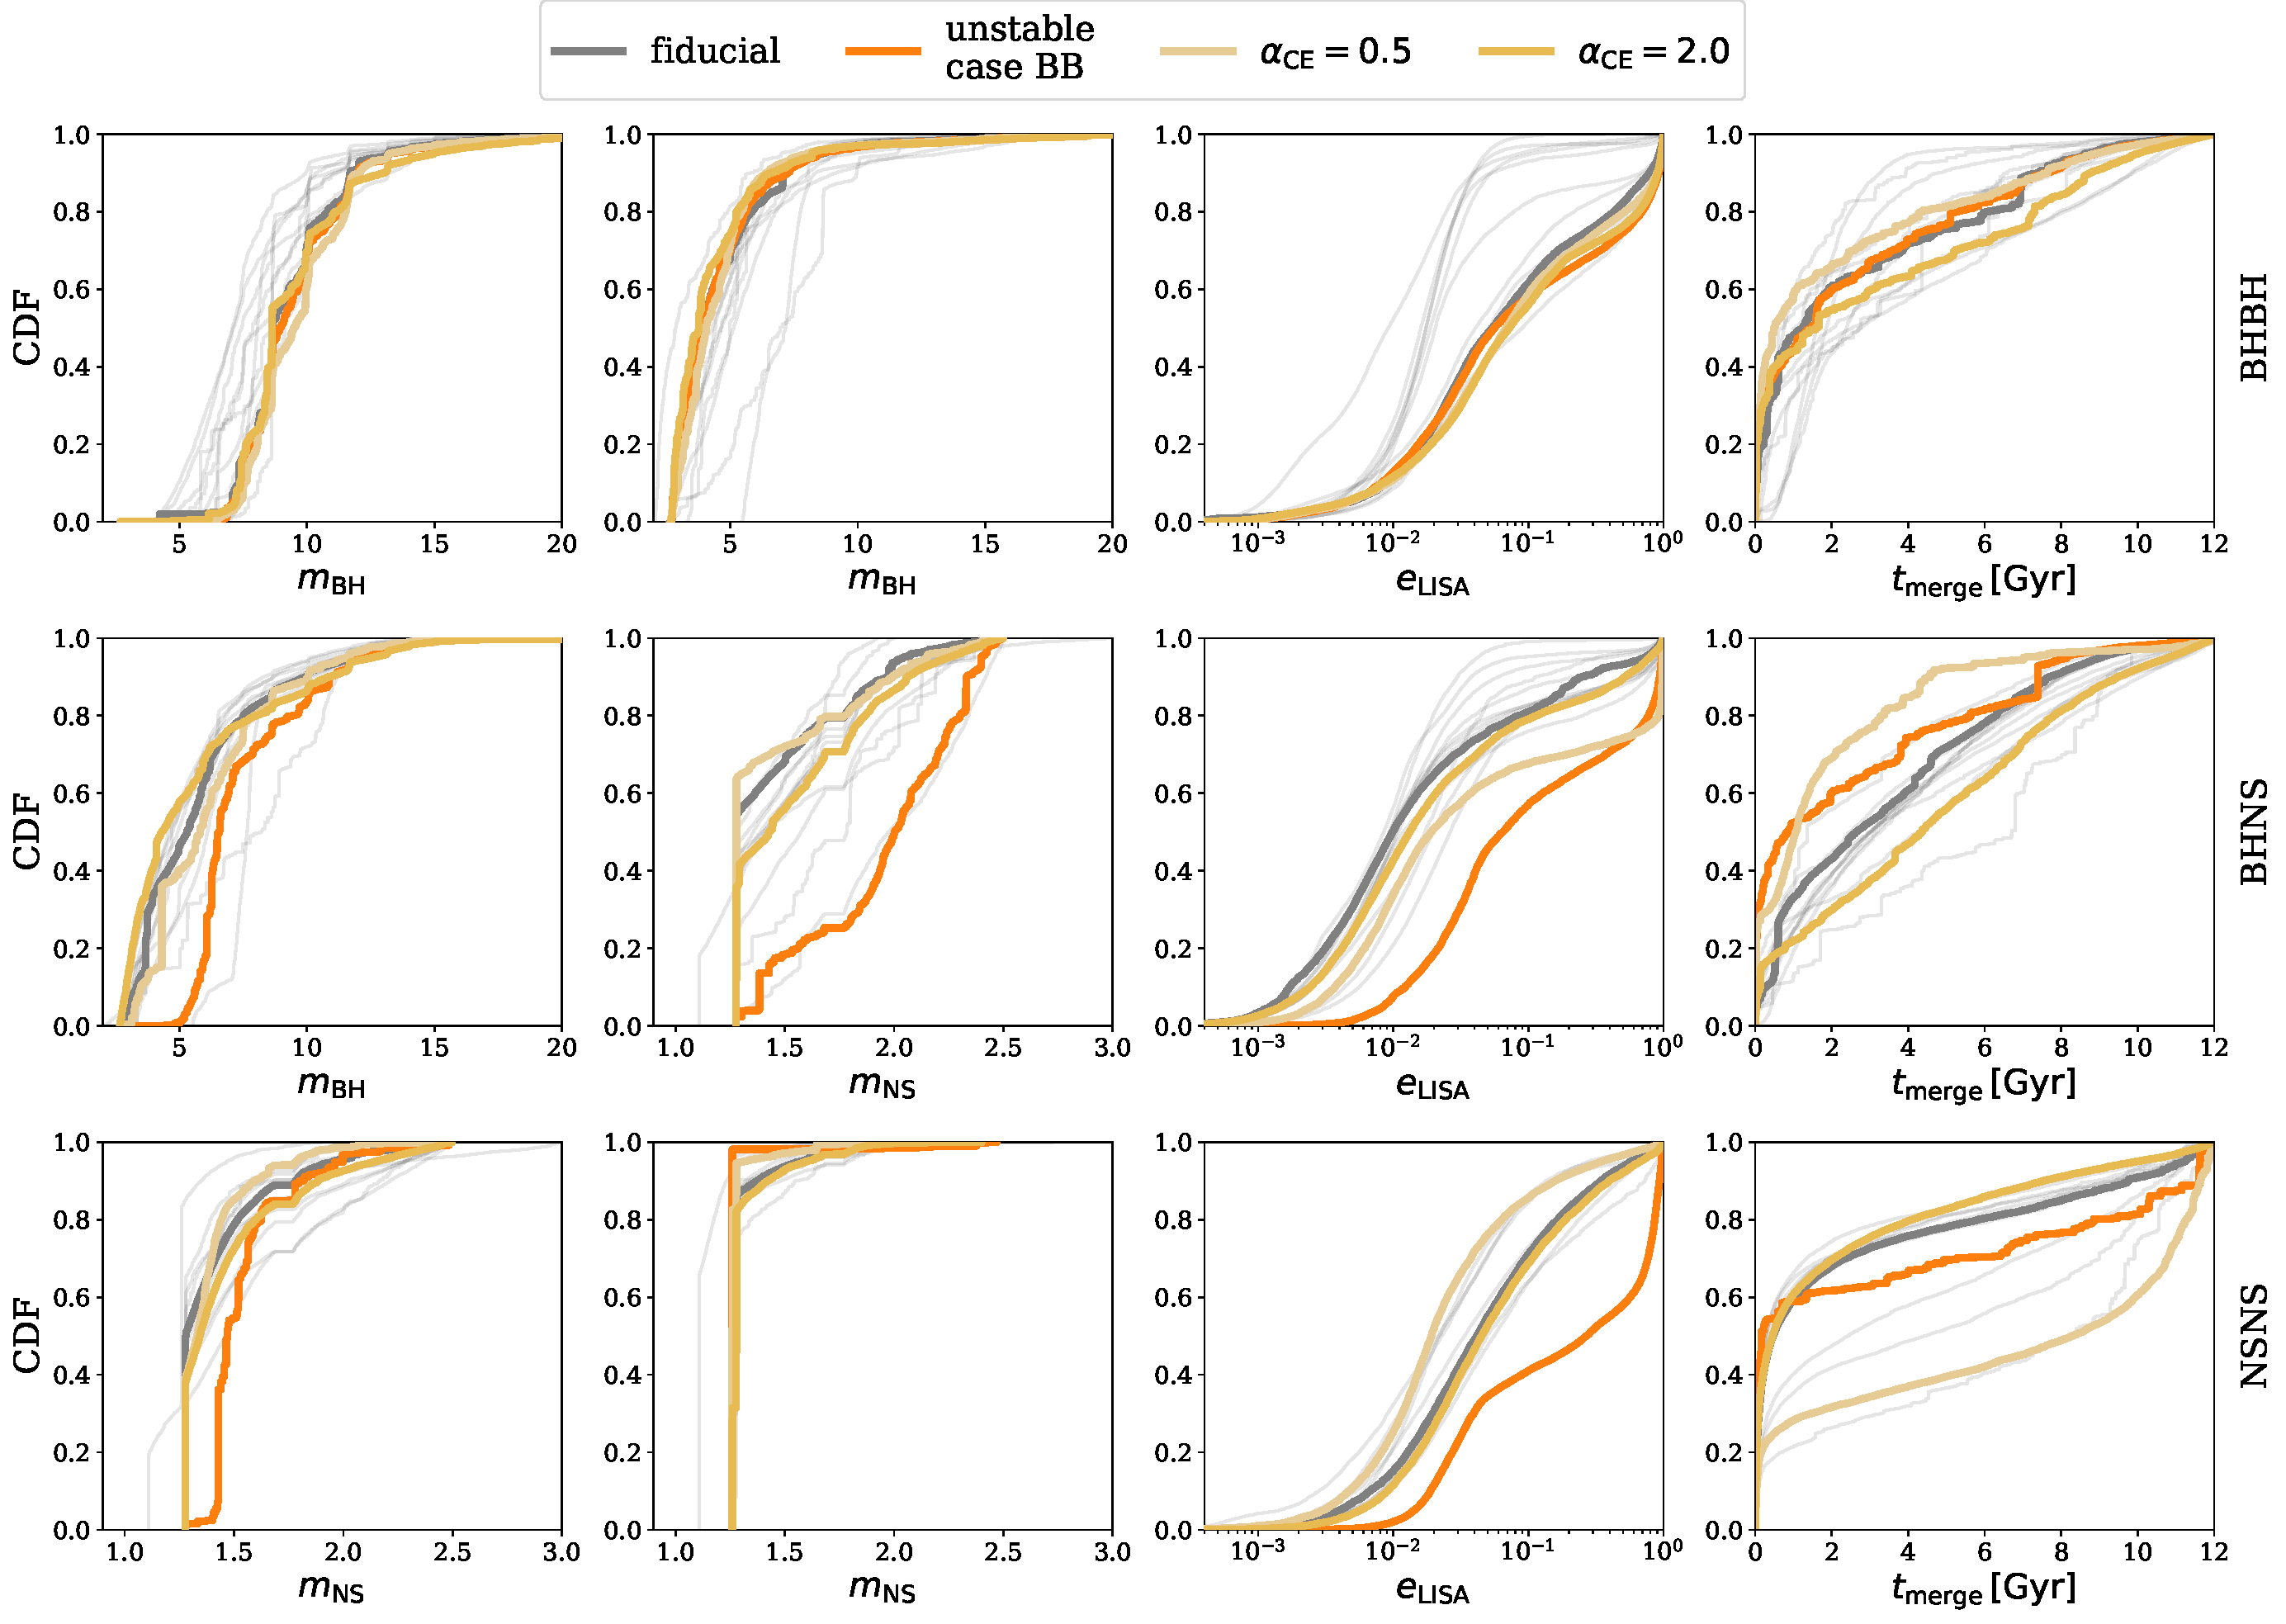
\includegraphics[width=\textwidth]{variations_cdf_4_6.pdf}
    \caption{As Fig.~\ref{fig:variations_cdf_1_3}, except comparing the fiducial population with models using different values for $\alpha_{\rm CE}$ and changing the stability of case BB mass transfer.}
    \label{fig:variations_cdf_4_6}
\end{figure*}

\begin{figure*}[h]
    \centering
    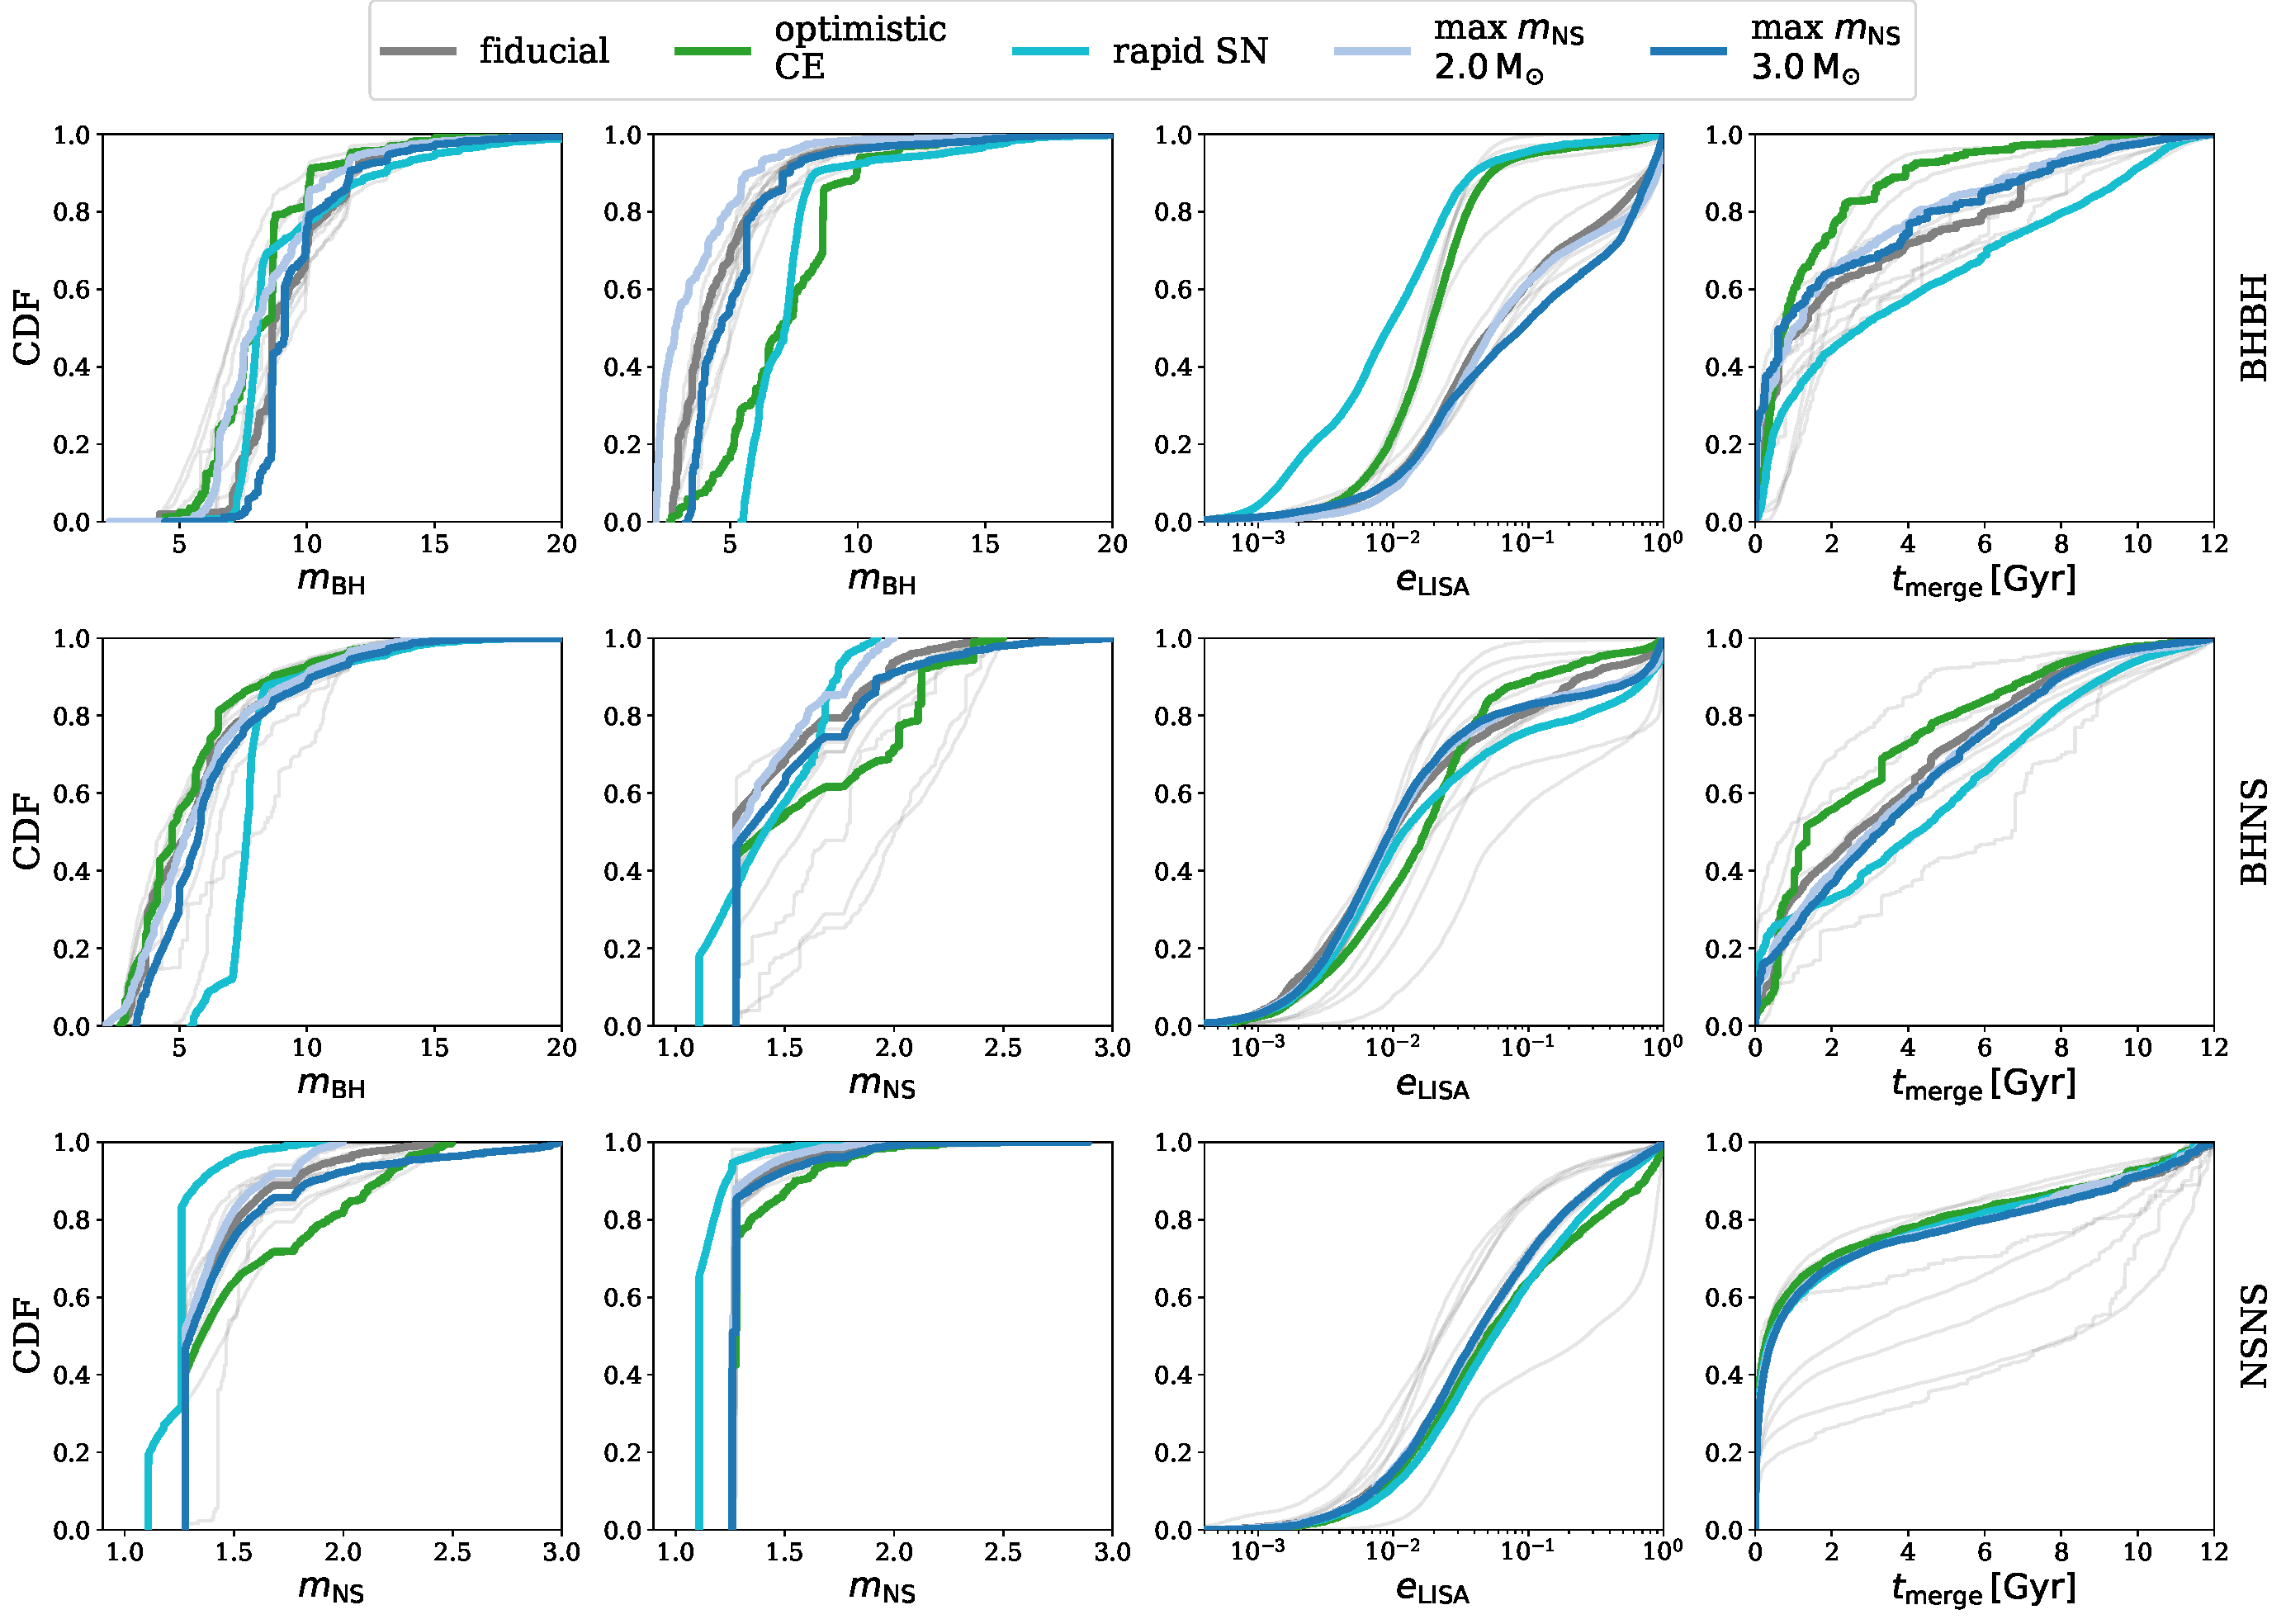
\includegraphics[width=\textwidth]{variations_cdf_7_10.pdf}
    \caption{As Fig.~\ref{fig:variations_cdf_1_3}, except comparing the fiducial population with models changing the maximum neutron star mass, remnant mass prescription and survivability of common envelope events initiated by Hertzsprung gap donors.}
    \label{fig:variations_cdf_7_10}
\end{figure*}

\begin{figure*}[h]
    \centering
    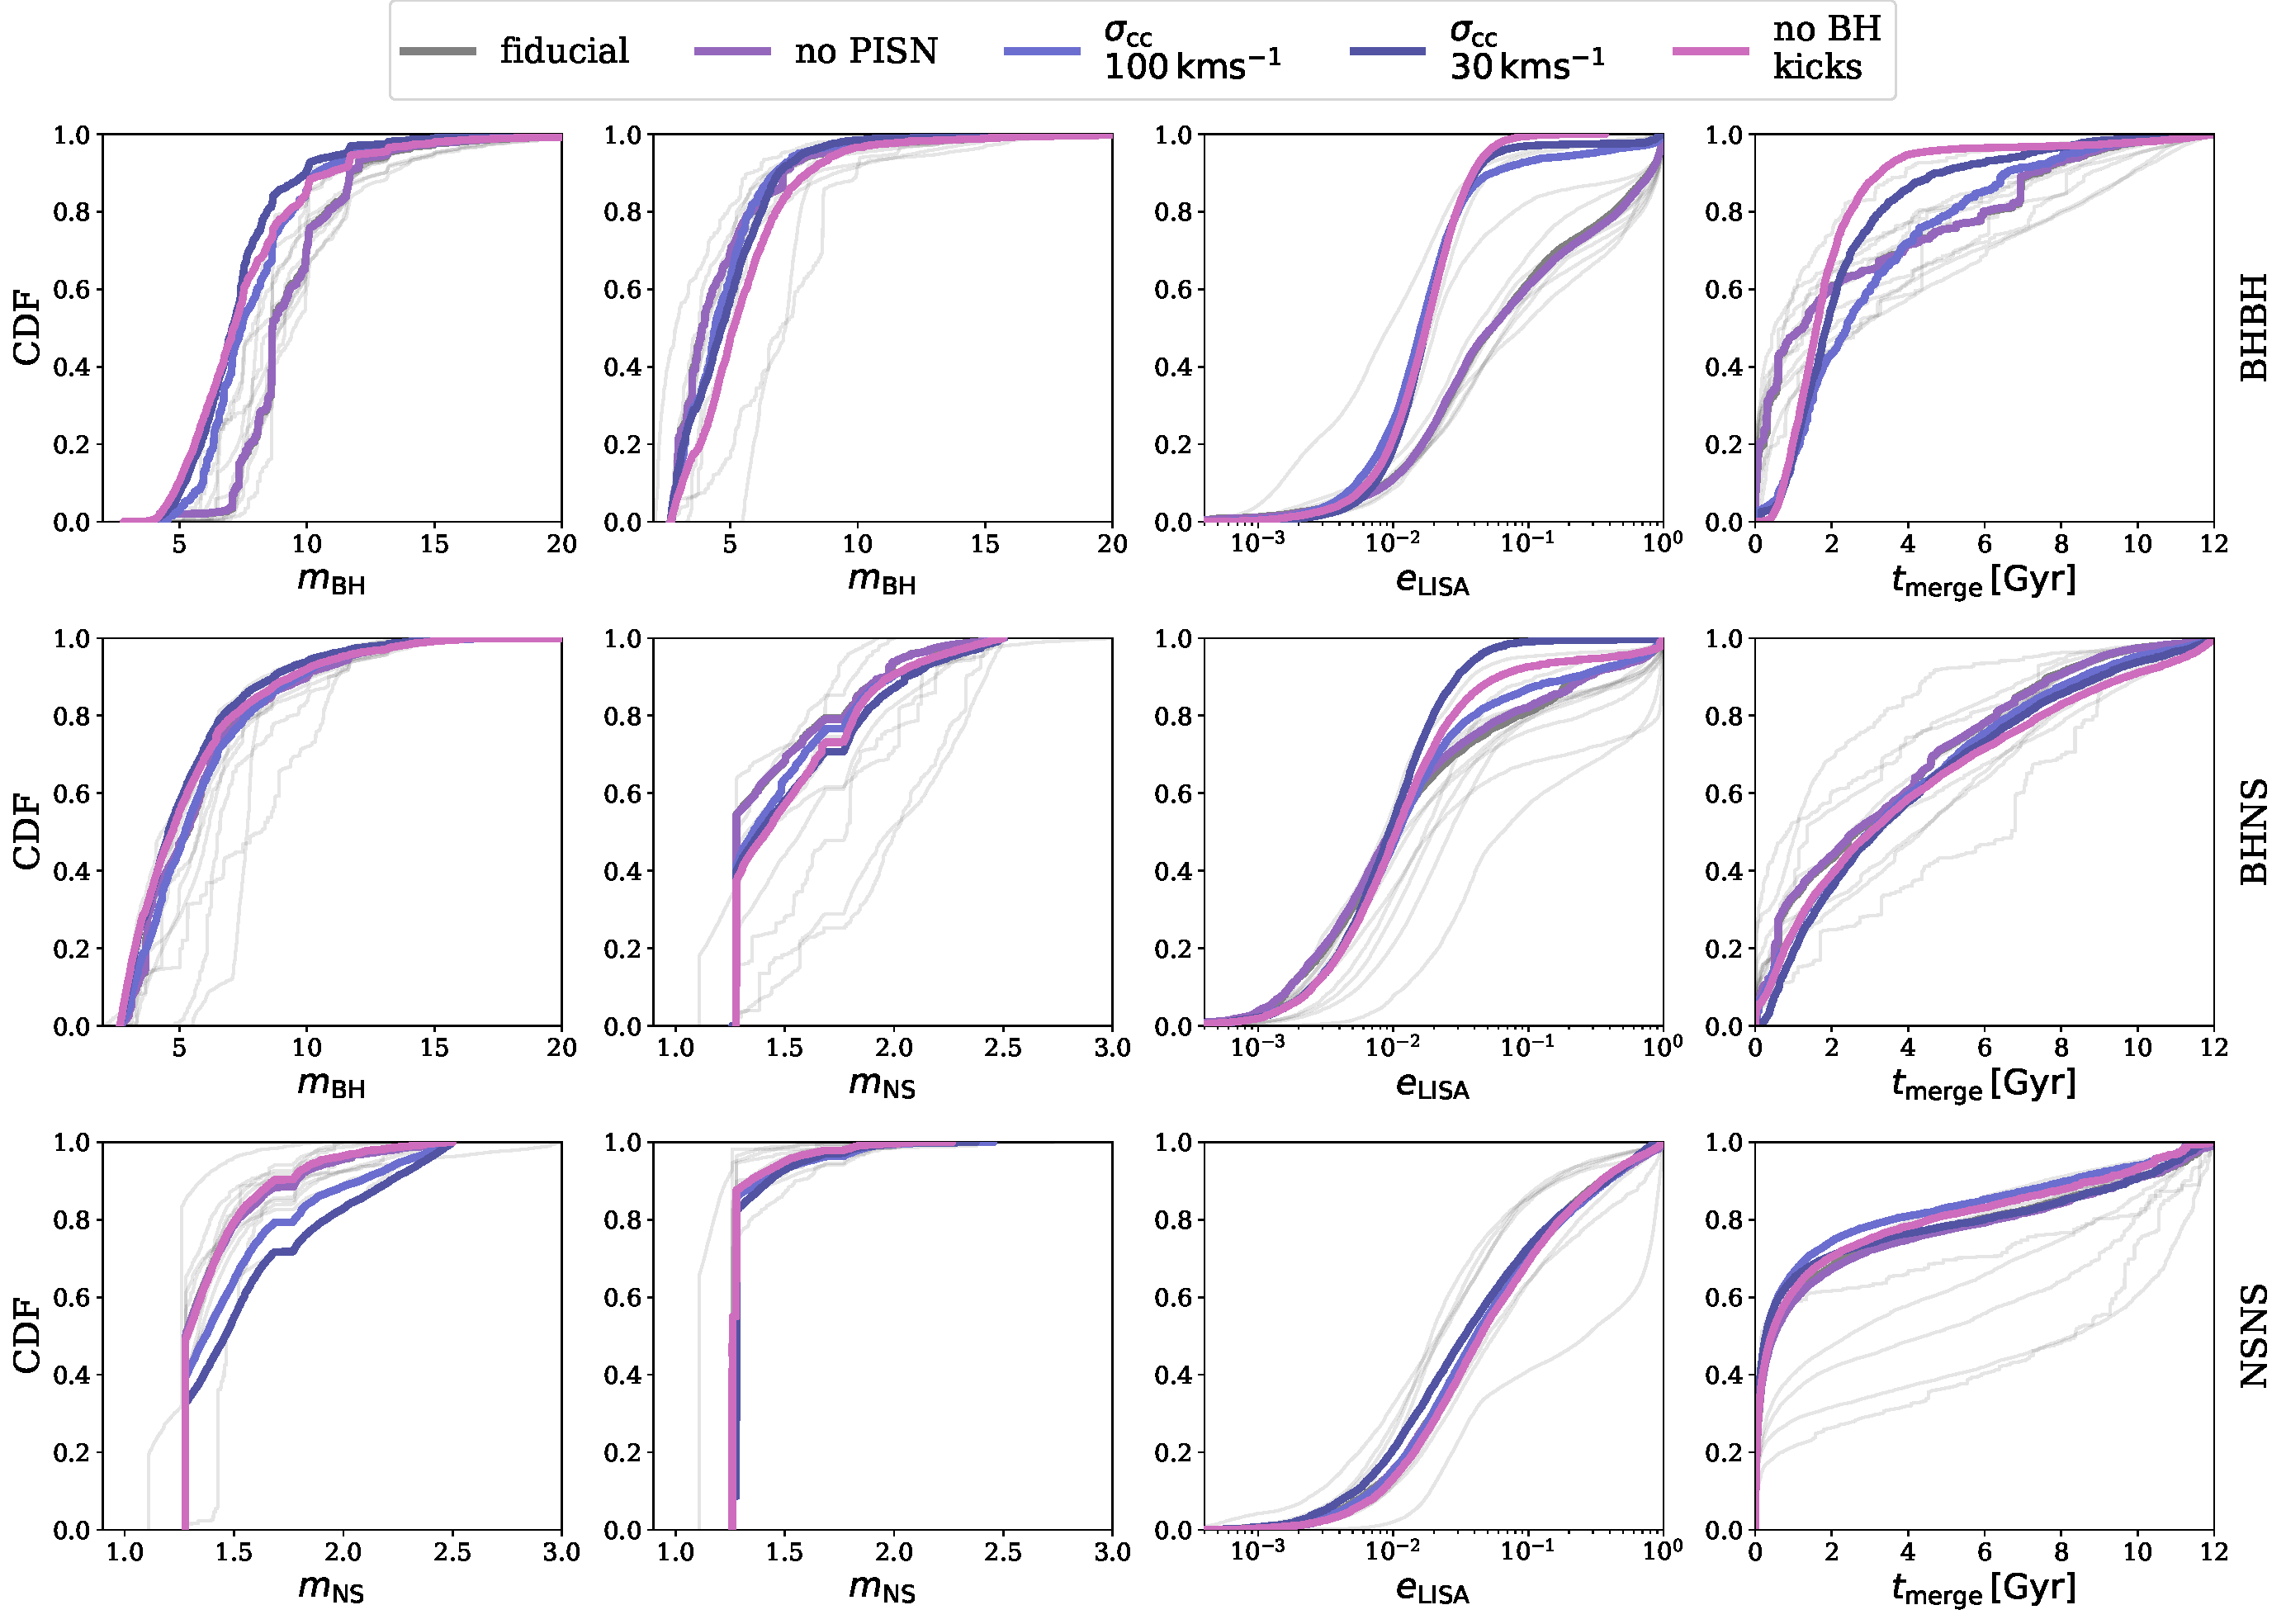
\includegraphics[width=\textwidth]{variations_cdf_11_14.pdf}
    \caption{As Fig.~\ref{fig:variations_cdf_1_3}, except comparing the fiducial population with models changing the core-collapse supernova kick distributions and the presence of BH kicks and PISNs.}
    \label{fig:variations_cdf_11_14}
\end{figure*}

\subsection{Formation channels}

\begin{figure}
    \centering
    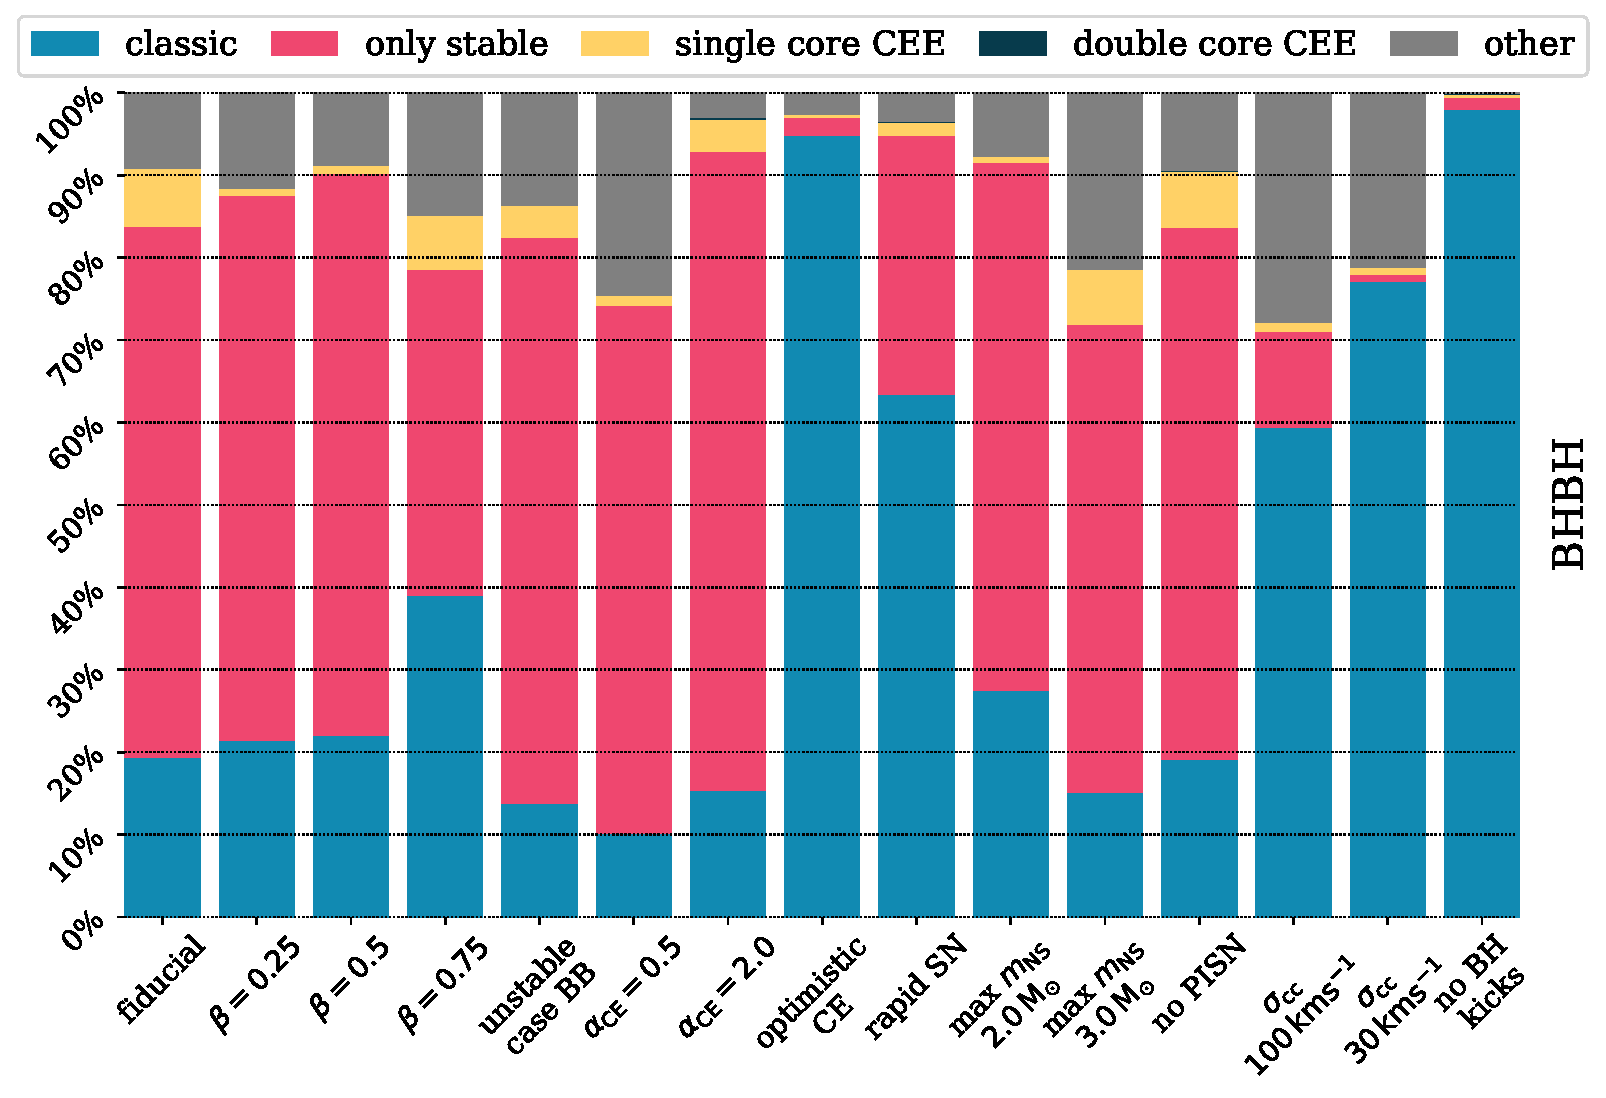
\includegraphics[width=\textwidth]{formation_channels_BHBH.pdf}
\end{figure}

\begin{figure}
    \centering
    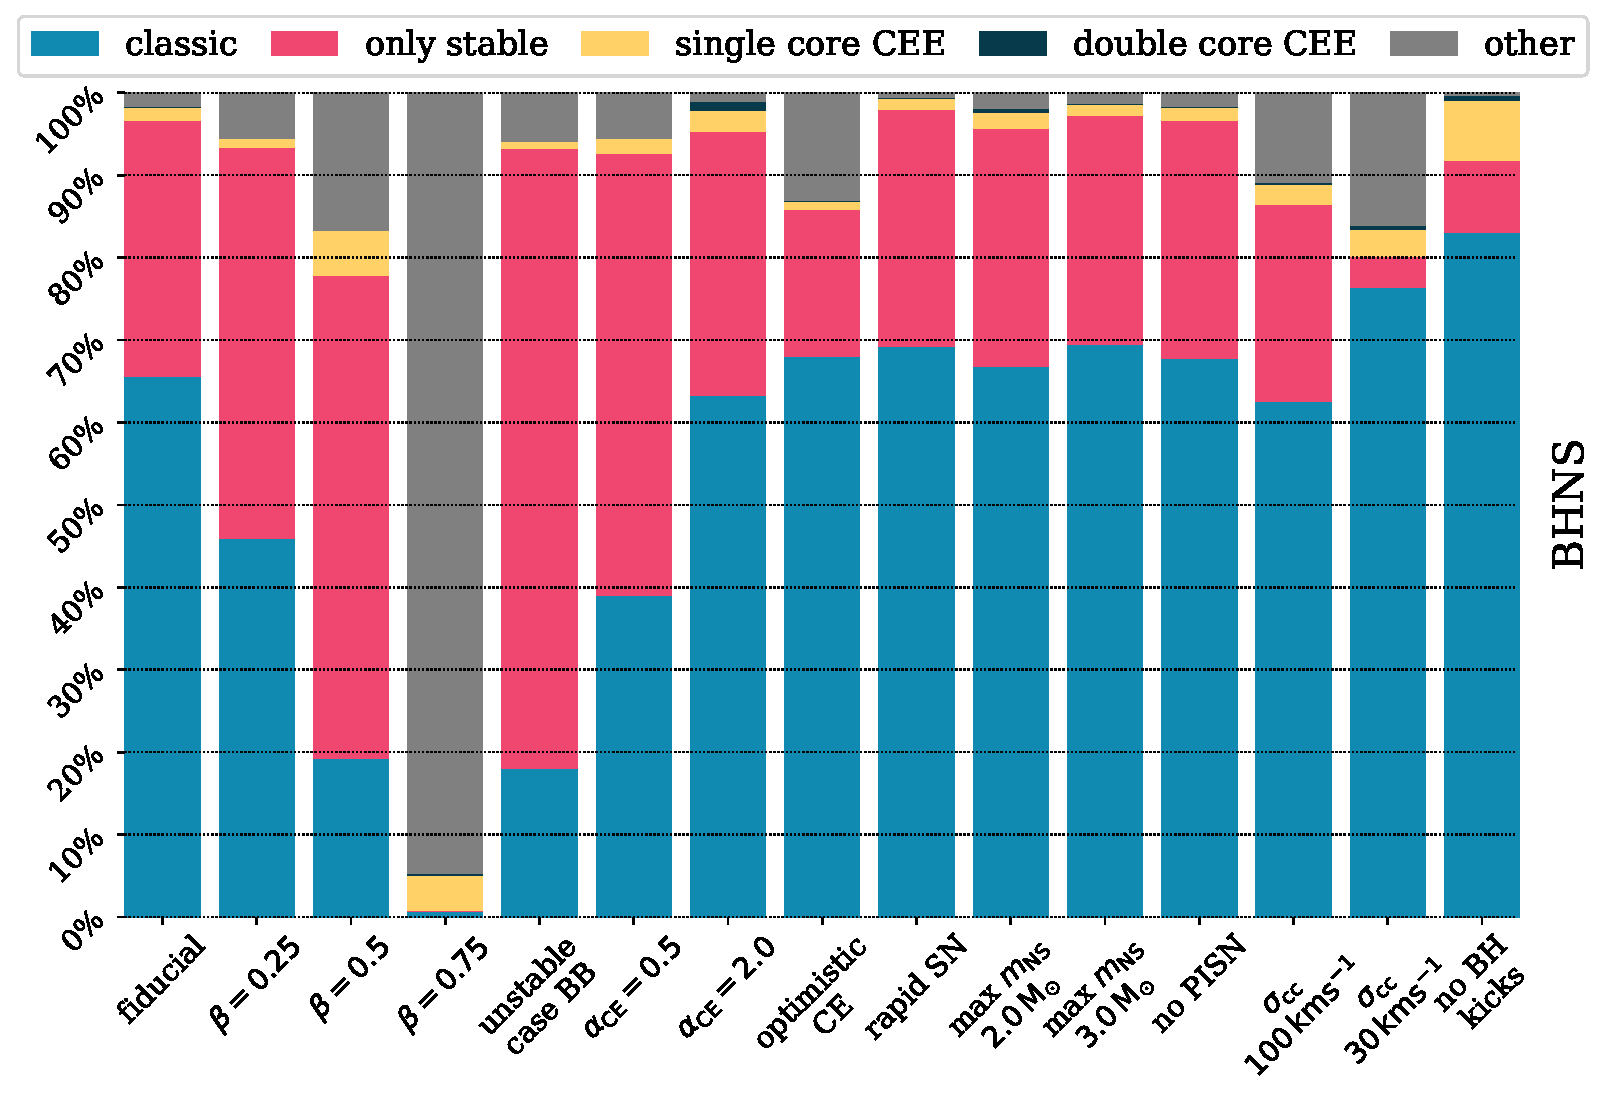
\includegraphics[width=\textwidth]{formation_channels_BHNS.pdf}
\end{figure}

\begin{figure}
    \centering
    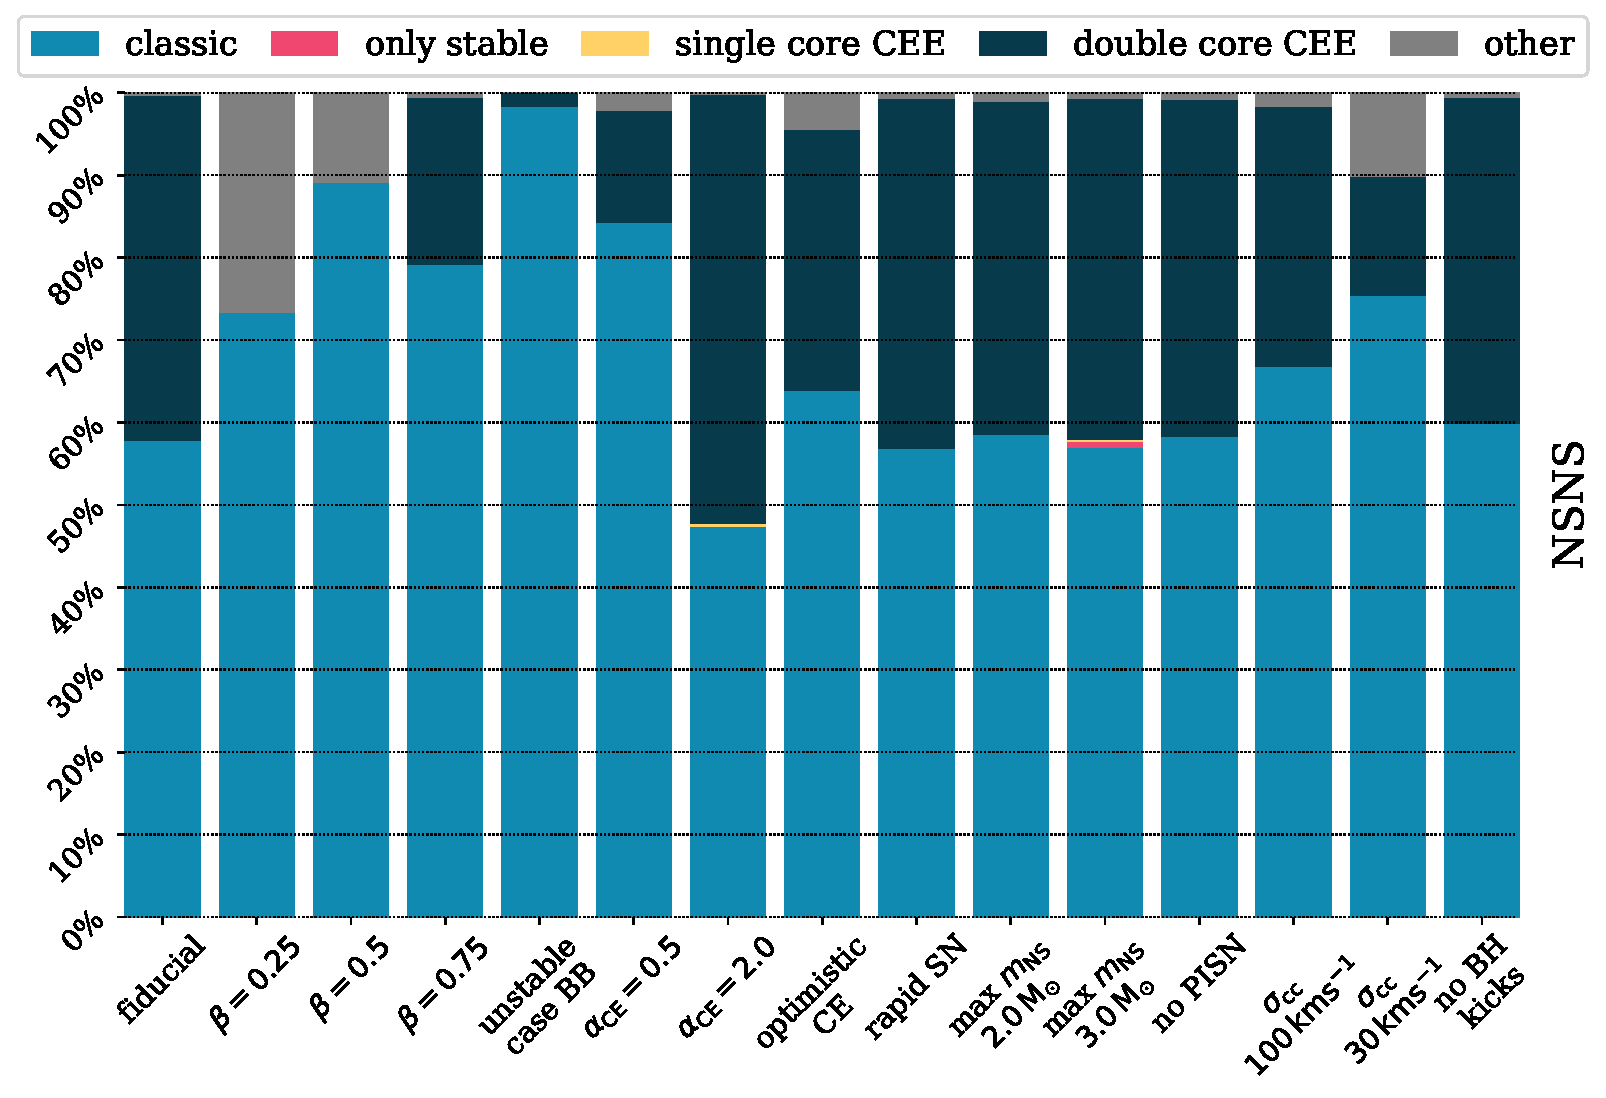
\includegraphics[width=\textwidth]{formation_channels_NSNS.pdf}
\end{figure}